\documentclass{article}

\usepackage[UTF8]{ctex}
\usepackage{amsmath,amssymb}
\usepackage{geometry}
\usepackage{graphicx}

\geometry{a4paper, margin=2.5cm}

\begin{document}

% ============================================================
\section*{马尔可夫决策过程（Markov Decision Process, MDP）}

\subsection*{先讲一个故事}

想象你是一只小老鼠，住在一个 $3\times 3$ 的迷宫里。你每次可以上、下、左、右走一步。走到奶酪格子得 $+1$ 分，走到电击格子得 $-1$ 分，其他格子不得分。你的目标是：找到一条路，让长期累积的分数最多。

这个故事就是一个 MDP。下面把故事里的要素翻译成数学语言。

\subsection*{数学形式化：五元组}

MDP 由五个要素完整描述：

\[
\boxed{\mathcal{M} = (\mathcal{S}, \mathcal{A}, \mathcal{P}, \mathcal{R}, \gamma)}
\]

\begin{itemize}
  \item $\mathcal{S}$ —— \textbf{状态空间}。所有可能状态的集合（迷宫例中 $\mathcal{S}=\{1,\ldots,9\}$ 九个格子）；
  \item $\mathcal{A}$ —— \textbf{动作空间}。所有可能动作的集合（$\mathcal{A}=\{\uparrow,\downarrow,\leftarrow,\rightarrow\}$，$|\mathcal{A}|=4$）；
  \item $\mathcal{P}$ —— \textbf{状态转移概率}。MDP 的 Markov 性质核心——下一状态只依赖当前状态与动作，与更早的历史无关：
        \[
        P(S_{t+1}=s' \mid S_t=s, A_t=a, S_{t-1}, A_{t-1},\ldots,S_0) = P(S_{t+1}=s' \mid S_t=s, A_t=a)
        \]
        简记 $P^{a}_{ss'} = P(s'\mid s,a)$。对任意 $s,a$，它构成一个分布：$\sum_{s'\in\mathcal{S}}P(s'\mid s,a)=1$；
  \item $\mathcal{R}$ —— \textbf{奖励函数}。$R(s,a)=\mathbb{E}[R_{t+1}\mid S_t=s, A_t=a]$ 是在状态 $s$ 采取动作 $a$ 后获得的即时奖励的期望（也可写成 $R(s,a,s')$ 形式）；
  \item $\gamma \in [0,1)$ —— \textbf{折扣因子}。$\gamma\to 0$ 只看眼前，$\gamma\to 1$ 注重长期累积；$\gamma<1$ 数学上保证无限时域回报级数收敛（若奖励有界）。
\end{itemize}

\subsection*{交互过程}

Agent 与环境在离散时间步 $t=0,1,2,\ldots$ 上交互，每一步产生一个四元组 $(S_t, A_t, R_{t+1}, S_{t+1})$，完整轨迹为：

\[
S_0, A_0, R_1, S_1, A_1, R_2, S_2, \ldots
\]

这个序列的联合分布由转移概率 $\mathcal{P}$ 和策略 $\pi$ 共同决定——这就是强化学习全部数据的来源：试错、拿反馈、调整、再来。

% ============================================================
\section*{价值函数——什么是「好」状态}

\subsection*{回报（Return）}

不能光看脚下一步的奖励——奶酪可能在隔壁，也可能在十步之外。定义\textbf{折扣回报}：

\[
\boxed{G_t = R_{t+1} + \gamma R_{t+2} + \gamma^2 R_{t+3} + \cdots = \sum_{k=0}^{\infty} \gamma^k R_{t+k+1}}
\]

把未来的所有奖励加起来，离现在越远折扣越重。其递归形式是后续所有 Bellman 推导的起点：

\[
\boxed{G_t = R_{t+1} + \gamma G_{t+1}}
\]

\subsection*{价值函数：回报的条件期望}

因为转移是随机的，你无法精确预测未来，只能求期望：

\[
\boxed{v_\pi(s) = \mathbb{E}_\pi[G_t \mid S_t = s]}, \qquad
\boxed{q_\pi(s,a) = \mathbb{E}_\pi[G_t \mid S_t = s, A_t = a]}
\]

\begin{itemize}
  \item $v_\pi(s)$ —— 给定策略 $\pi$，从状态 $s$ 出发平均能拿多少回报（\textbf{状态价值}）；
  \item $q_\pi(s,a)$ —— 在状态 $s$ 先执行动作 $a$，之后按 $\pi$ 行动，平均能拿多少回报（\textbf{动作价值}）。
\end{itemize}

一句话：价值不是精确的未来，而是对未来回报的条件期望。

\subsection*{$v_\pi$ 与 $q_\pi$ 的关系}

由定义立即可得二者互推：

\[
v_\pi(s) = \sum_{a\in\mathcal{A}} \pi(a\mid s)\, q_\pi(s,a)
\]
\[
q_\pi(s,a) = R(s,a) + \gamma \sum_{s'\in\mathcal{S}} P(s'\mid s,a)\, v_\pi(s')
\]

状态价值 = 按策略对动作价值加权平均；动作价值 = 即时奖励 + 折扣后后继状态价值的期望。这两个关系在后面推导 Bellman 方程时反复用到。

% ============================================================
\section*{Bellman 期望方程——把未来拆成「眼前 + 之后」}

\subsection*{推导}

Bellman 的关键发现是：价值可以\textbf{递归}地定义。从 $G_t = R_{t+1} + \gamma G_{t+1}$ 出发：

\[
\begin{aligned}
v_\pi(s) &= \mathbb{E}_\pi[G_t \mid S_t=s] \\
&= \mathbb{E}_\pi[R_{t+1} + \gamma G_{t+1} \mid S_t=s] \\
&= \mathbb{E}_\pi[R_{t+1}\mid S_t=s] + \gamma\,\mathbb{E}_\pi[G_{t+1}\mid S_t=s]
\end{aligned}
\]

第一项是即时奖励的期望，第二项是后继价值的期望。对动作 $a$ 与后继状态 $s'$ 展开求和：

\[
\boxed{v_\pi(s) = \sum_{a\in\mathcal{A}} \pi(a\mid s) \left[ R(s,a) + \gamma \sum_{s'\in\mathcal{S}} P(s'\mid s,a)\, v_\pi(s') \right]}
\]

它说：你不需要看无限远的未来，只需看一步，然后用下一个状态的价值估计余下的。动作价值的 Bellman 期望方程同理：

\[
q_\pi(s,a) = R(s,a) + \gamma \sum_{s'\in\mathcal{S}} P(s'\mid s,a) \sum_{a'\in\mathcal{A}} \pi(a'\mid s')\, q_\pi(s',a')
\]

\subsection*{一个具体例子}

假设你在格子 A，往右走必到格子 B，奖励 $R=0$。若 $v(B)=5$，$\gamma=0.9$：

\[
q(A, \rightarrow) = 0 + 0.9 \times 5 = 4.5
\]

格子 A 本身没奖励，但因为右边是「好地方」，A 也是好地方。这就是 Bellman 方程的直观威力——价值通过递归在状态间传播。

\subsection*{矩阵形式（有限状态 MDP）}

状态空间有限时，Bellman 期望方程是线性方程组：

\[
\boxed{v_\pi = R_\pi + \gamma P_\pi v_\pi}
\]

其中 $v_\pi\in\mathbb{R}^{|\mathcal{S}|}$，$R_\pi(s)=\sum_a \pi(a\mid s)R(s,a)$，$P_\pi(s,s')=\sum_a \pi(a\mid s)P(s'\mid s,a)$。可直接求闭式解：

\[
v_\pi = (I - \gamma P_\pi)^{-1} R_\pi
\]

这是唯一能写闭式解的地方——最优方程就没有这么幸运了。

% ============================================================
\section*{Bellman 最优方程——每一步都选最好的}

\subsection*{最优价值函数}

定义最优价值函数为所有策略中的最大值：

\[
v_*(s) = \max_\pi v_\pi(s),\quad \forall s\in\mathcal{S}, \qquad
q_*(s,a) = \max_\pi q_\pi(s,a),\quad \forall s\in\mathcal{S},\, a\in\mathcal{A}
\]

对有限 MDP，最优策略 $\pi_*$ 一定存在且满足 $v_{\pi_*}=v_*$（逐状态）；并有 $v_*(s)=\max_a q_*(s,a)$。

\subsection*{状态价值的最优方程推导}

把 Bellman 期望方程中的「按策略加权平均」换成「取最大」：

\[
\boxed{v_*(s) = \max_{a\in\mathcal{A}} \left[ R(s,a) + \gamma \sum_{s'\in\mathcal{S}} P(s'\mid s,a)\, v_*(s') \right]}
\]

更严格地从定义出发：设 $\pi_*$ 为最优策略，则 $v_{\pi_*}=v_*$、$q_{\pi_*}=q_*$。把 $v_* = v_{\pi_*}$ 代入动作价值的 Bellman 期望方程 $q_*(s,a) = R(s,a) + \gamma\sum_{s'}P(s'\mid s,a)\,v_*(s')$，再利用 $v_* = \max_a q_*$ 对 $a$ 取最大：

\[
v_*(s) = \max_a q_*(s,a) = \max_a \left[ R(s,a) + \gamma \sum_{s'\in\mathcal{S}} P(s'\mid s,a)\, v_*(s') \right]
\]

和期望方程的区别只有一个：$\sum_a \pi(a\mid s)$ 换成了 $\max_a$。动作价值的最优方程：

\[
q_*(s,a) = R(s,a) + \gamma \sum_{s'\in\mathcal{S}} P(s'\mid s,a) \max_{a'\in\mathcal{A}} q_*(s',a')
\]

\subsection*{为什么没有闭式解？}

Bellman 期望方程是线性的（可求逆），最优方程却是\textbf{非线性的}——$\max$ 算子破坏了线性结构，无法求逆，只能迭代逼近：

\[
\begin{aligned}
&v_\pi = R_\pi + \gamma P_\pi v_\pi \;\Longrightarrow\; v_\pi = (I-\gamma P_\pi)^{-1}R_\pi \qquad \text{（线性，可求逆）}\\
&v_* = \max_a \left(R_a + \gamma P_a v_*\right) \qquad \text{（非线性，含 $\max$，无法求逆）}
\end{aligned}
\]

这就是下一节动态规划（值迭代、策略迭代）出现的原因。

% ============================================================
\section*{从方程到算法：策略提升与动态规划}

\subsection*{策略提升定理}

给定任意策略 $\pi$ 与它的 $q_\pi$，构造新策略 $\pi'(s) = \arg\max_a q_\pi(s,a)$，则 $\pi'$ \textbf{不差于} $\pi$（即 $v_{\pi'} \ge v_\pi$ 逐分量成立），这称为\textbf{策略提升定理}。反复交替「评估 → 提升」至不动点，即收敛到最优策略 $\pi_*$。

\subsection*{动态规划三件套}

已知模型 $\mathcal{P}$、$\mathcal{R}$ 时，可以精确求解 MDP。三套算法在 $4\times 4$ GridWorld（右下角为目标格，进入得 $+1$，$\gamma=0.9$）上的行为如下。

\textbf{策略评估}：迭代 Bellman 期望方程 $V_{k+1}(s) \leftarrow \sum_a \pi(a\mid s)\bigl[R(s,a)+\gamma\sum_{s'}P(s'\mid s,a)V_k(s')\bigr]$，收敛到 $v_\pi$。图~\ref{fig:policy-eval} 左图展示几个状态的 $V_k(s)$ 随扫描收敛，右图为收敛后的 $v_\pi$ 热力图。

\begin{figure}[!htbp]
  \centering
  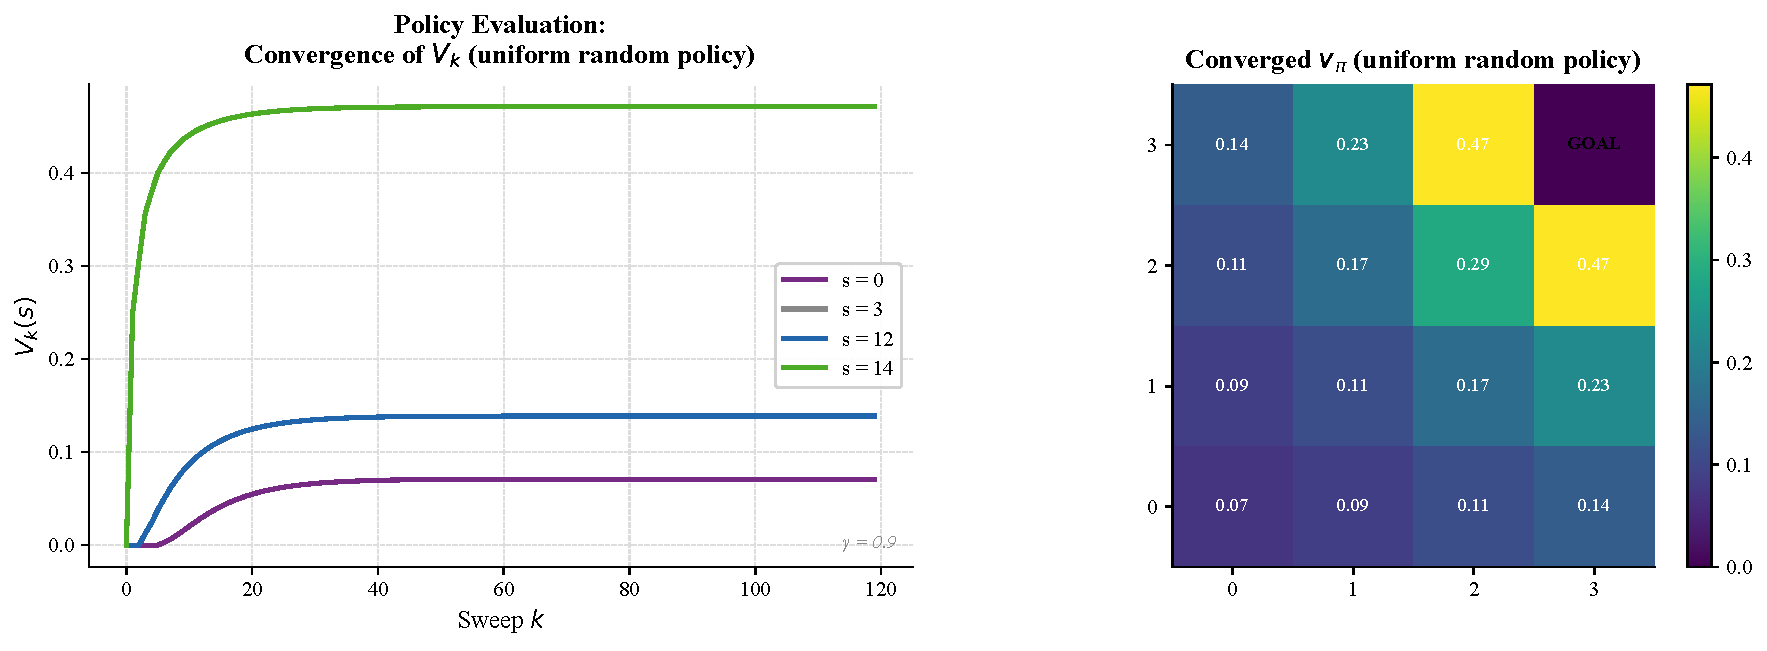
\includegraphics[width=0.85\textwidth]{fig1_policy_evaluation.pdf}
  \caption{策略评估（$4\times4$ GridWorld，均匀随机策略，$\gamma=0.9$）。左：四个状态的 $V_k(s)$ 随扫描次数收敛（紧邻目标的格收敛快、远角格收敛慢）；右：收敛后 $v_\pi$ 的热力图。}
  \label{fig:policy-eval}
\end{figure}

\textbf{值迭代}：迭代 Bellman 最优方程 $V_{k+1}(s) \leftarrow \max_a\bigl[R(s,a)+\gamma\sum_{s'}P(s'\mid s,a)V_k(s')\bigr]$。图~\ref{fig:vi-wave} 显示高价值区域像水波一样从目标格逐轮向外扩展。

\begin{figure}[!htbp]
  \centering
  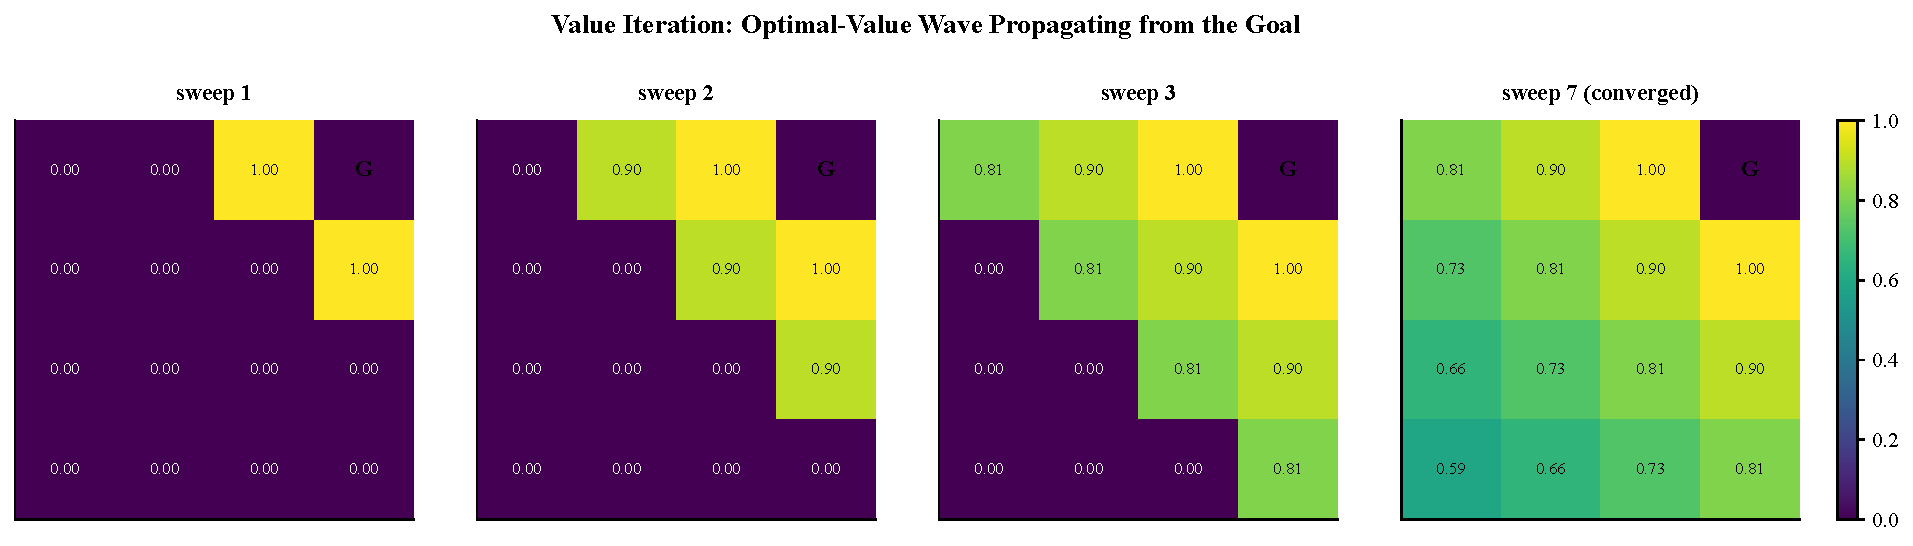
\includegraphics[width=0.85\textwidth]{fig2_value_iteration_wave.pdf}
  \caption{值迭代的价值传播（$4\times4$ GridWorld，$\gamma=0.9$）。第 1/2/3 轮与收敛时（第 7 轮）的 $V_k$：一步可达目标格的格价值最先变为 $1.0$，之后每多一轮价值向外辐射一格。}
  \label{fig:vi-wave}
\end{figure}

\textbf{策略迭代}：交替「完整策略评估 → 贪心改进」。图~\ref{fig:pi-vi} 对比两种算法的收敛动态。

\begin{figure}[!htbp]
  \centering
  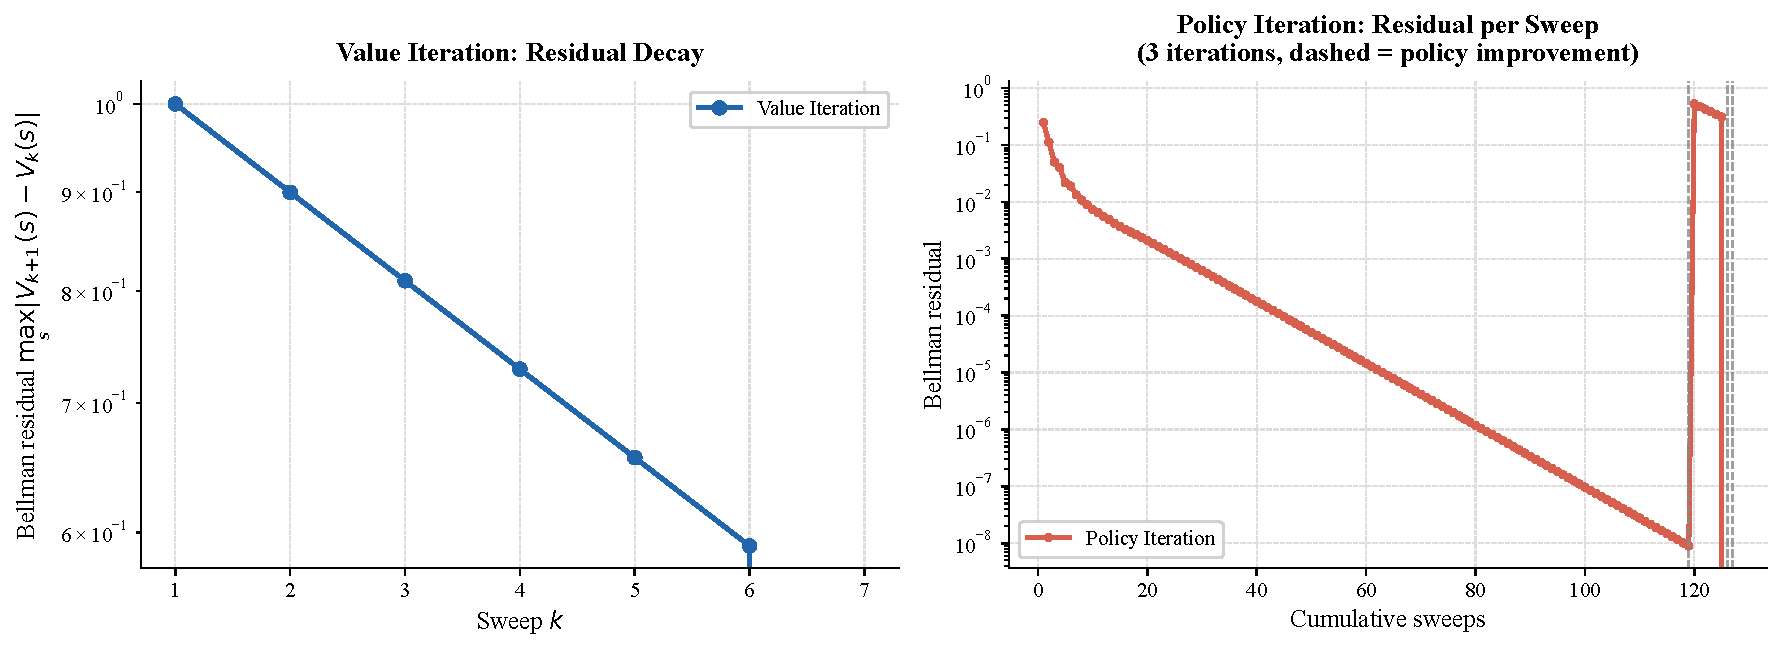
\includegraphics[width=0.88\textwidth]{fig3_policy_vs_value_iteration.pdf}
  \caption{值迭代 vs 策略迭代（$4\times4$ GridWorld，$\gamma=0.9$）。左：值迭代的 Bellman 残差 $\max_s|V_{k+1}-V_k|$ 单调几何衰减（本例 7 轮收敛）；右：策略迭代的残差逐扫描呈阶梯下降（虚线为每次策略改进，本例 3 轮迭代、约 127 轮扫描）。两种算法收敛到同一个 $V^*$（数值上 $\max_s|V^{VI}_*-V^{PI}_*|=0$）。}
  \label{fig:pi-vi}
\end{figure}

\textbf{共性}：三者都需要\textbf{已知模型}——DP 用 $P(s'\mid s,a)$ 对所有后继求期望。现实中模型往往未知，这正是下一章 TD 学习要打破的假设。

% ============================================================
\section*{本章在 RL 体系中的位置}

\begin{enumerate}
  \item \textbf{上游}：MAB 教会我们探索 vs.\ 利用与增量更新 $\theta \leftarrow \theta+\alpha(\text{Target}-\theta)$；
  \item \underline{\textbf{本章（MDP）}}：把单状态扩展为带转移的序列决策，用 $(\mathcal{S},\mathcal{A},\mathcal{P},\mathcal{R},\gamma)$ 五元组、价值函数与 Bellman 方程搭起整个 RL 的理论骨架；
  \item \textbf{下游}：Bellman 方程是后面一切的递归根基——TD 学习把「对所有后继求期望」换成「采样一次」；DQN 用神经网络逼近 $Q$；策略梯度直接在策略空间优化。
\end{enumerate}

学完本章，你应该能看懂任何 MDP 的「问题定义」，并且理解价值函数为什么可以递归定义、最优方程为什么没有闭式解。下一章进入 TD 学习：去掉「已知模型」这个最强假设。

\subsection*{参考资料}

\begin{enumerate}
  \item Sutton \& Barto (2018). \textit{Reinforcement Learning: An Introduction} (2nd ed.). Chapters 3--4.
  \item Bellman, R. (1957). \textit{Dynamic Programming}. Princeton University Press.
  \item Puterman, M. L. (1994). \textit{Markov Decision Processes}. Wiley.
  \item 动手学强化学习（Hands-on-RL）. 第 3 章：马尔可夫决策过程.
\end{enumerate}

\end{document}
